\section{CSS Exercises} \label{sect:css-exercises}

\subsection*{Exercise 1}
\coderef{code:exercise-selectors-1}가 \figref{fig:exercise-selectors-1}과 같이 나타나도록 style.3.1.css를 작성하여라.

\figcmd{fig:exercise-selectors-1}{Exercise 1 Example}
    {images/css-designing-html/exercise-selectors-1.png}{0.65}


\begin{codeenv}{code:exercise-selectors-1}{Exercise 1}\begin{verbatim}
    

<!doctype html>
<html>
<head>
    <title>CSS Exercise 1</title>
    <meta charset="utf-8">
    <link rel="stylesheet" text="type/css" href="./style.3.1.css">
</head>
<body>
    <h1>Chapters</h1>
    <div class="horizontal-lists">
        Ch 2. HTML: The Basic Structure / Ch 3. CSS: Desiging HTML
        / Ch 4. Basics of Javascript
    </div><br>
    <div class="chapter">
        <div class="chapter-name">Ch 2. HTML: The Basic Structure</div>
        <div class="horizontal-lists">
            Introducing HTML / Basic Structure of HTML / Commonly Used HTML Tags
        </div>
    </div><br>
    <div class="chapter" id="current-chapter">
        <div class="chapter-name">Ch 3. CSS: Desiging HTML</div>
        <div class="horizontal-lists">
            Introducing CSS / Basic Structure of CSS / Selectors
        </ul>
    </div><br>
    <div class="chapter">
        <div class="chapter-name">Ch 4. Basics of Javascript</div>
        <div class="horizontal-lists">
            Introducing Javascript / Declaration of Variables / Data Types
        </div>
    </div>
</body>
</html>
\end{verbatim}
\end{codeenv}

\subsection*{Exercise 2}

\coderef{code:exercise-layouts-1}이 \figref{fig:exercise-layouts-1}과 같이 나타나도록 style.3.2.css를 작성하여라.

\figcmd{fig:exercise-layouts-1}{Exercise 2 Example}
    {images/css-designing-html/exercise-layouts-1.png}{.75}

\begin{codeenv}{code:exercise-layouts-1}{Exercise 2}\begin{verbatim}


<!doctype html>
<html>
<head>
    <title>CSS Exercise 2</title>
    <meta charset="utf-8">
    <link rel="stylesheet" text="type/css" href="./style.3.2.css">
</head>
<body>
    <div class="container" style="width: 500px">
        <div class="header">
            Click button you heard from ARS, then press submit button.
        </div>
        <div class="numbers">
            <div class="number">52</div>
            <div class="number">15</div>
            <div class="number">73</div>
            <div class="number">09</div>
            <div class="number">36</div>
        </div>
        <div class="footer">
            <button type="submit">Submit</button>
        </div>
    </div>
</body>
</html>
\end{verbatim}
\end{codeenv}

\subsection*{Exercise 3}

\coderef{code:exercise-layouts-2}을 참고하여, \figref{fig:exercise-layouts-2}과 같이 우측 하단에 고정되어 있으면서, 클릭하였을 때 웹 페이지의 제일 상단과 제일 하단으로 이동하는 버튼을 \texttt{\#scroll-button} 내부를 수정하고, style.3.3.css를 작성하여 구현하여라. \texttt{a} 태그의 \texttt{href} 속성값으로 HTML 요소의 Id를 주면 눌렀을 때 해당 위치로 이동할 수 있으며, 위쪽 삼각형(▲)과 아래쪽 삼각형(▼)의 개체 번호는 각각 9650, 9660이다.

\figcmd{fig:exercise-layouts-2}{Exercise 3 Example}
    {images/css-designing-html/exercise-layouts-2.png}{1.0}

\begin{codeenv}{code:exercise-layouts-2}{Exercise 3}\begin{verbatim}


<!doctype html>
<html>
<head>
    <title>CSS Exercise 3</title>
    <meta charset="utf-8">
    <link rel="stylesheet" text="type/css" href="./style.3.3.css">
    <style> #content { padding: 30px 100px; margin: 0 auto }
        #scroll-button a { text-decoration: none; }
        ul { margin: 20px 0 } li { margin: 10px 0 } </style>
</head>
<body>
    <div id="page-top"></div>
    <div id="content"><ul>
        <li>1 Introduction to Front-end</li>
        <ul><li>1.1 Introducing WEB</li><li>1.2 2021 Study Schedule</li>
            <li>1.3 Setting Development Environment</li></ul>
        <li>2 HTML: The Basic Structure</li>
        <ul><li>2.1 Introducing HTML</li><li>2.2 Basic Structure of HTML</li>
            <li>2.3 Commonly Used HTML Tags</li><li>2.4 Class and Id Attributes</li>
            <li>2.5 HTML Exercises</li></ul>
        <li>3 CSS: Desinging HTML</li>
        <ul><li>3.1 Introducing CSS</li><li>3.2 Basic Structure of CSS</li>
            <li>3.3 Style Properties</li><li>3.4 Selectors</li> <li>3.5 Layouts</li>
            <li>3.6 Responsive Web</li><li>3.7 CSS Exercises</li></ul>
        <li>4 Basics of Javascript</li>
        <ul><li>4.1 Introducing Javascript</li><li>4.2 Declaration of Variables</li>
            <li>4.3 Data Types</li><li>4.4 Statements and Functions</li>
            <li>4.5 Objects</li></ul>
        <li>5 Javascript: Dynamic Frontend</li>
        <ul><li>5.1 Javscript with Front-end</li> <li>5.2 Document Object Model</li>
            <li>5.3 Browser Object Model</li><li>5.4 Event and Event Listener</li>
            <li>5.5 JS Exercises</li></ul>
        <li>A Exercise Answers</li>
        <ul><li>A.1 HTML Exercise Answers</li><li>A.2 CSS Exercise Answers</li>
            <li>A.3 Basics of Javascript Exercise Answers</li>
            <li>A.4 JS Exercise Answers</li></ul>
    </ul></div>
    <div id="page-bottom"></div>
    <div id="scroll-button">
        <!-- Your code here -->
    </div>
</body>
</html>    
\end{verbatim}
\end{codeenv}

\subsection*{Exercise 4}
\coderef{code:exercise-responsive-web-1}를 참고하여, \texttt{body} 태그의 배경색을 800px 미만일 때는 \texttt{skyblue}, 800px 이상 1200px 미만일 때는 \texttt{blue}, 1200px 이상일 때는 \texttt{darkblue}가 되도록 style.3.4.css를 작성하여라. \texttt{h1} 태그의 색은 \texttt{white}로 고정되어야 한다.

\begin{codeenv}{code:exercise-responsive-web-1}{Exercise 4}\begin{verbatim}


<!doctype html>
<html>
<head>
    <title>CSS Exercise 4</title>
    <meta charset="utf-8">
    <meta name="viewport" content="width=device-width, initial-scale=1" >
    <link rel="stylesheet" text="type/css" href="./style.3.4.css">
</head>
<body>
    <h1 style="color: white">Responsive Web</h1>
</body>
</html>
\end{verbatim}
\end{codeenv}

\subsection*{Exercise 5}
\coderef{code:exercise-responsive-web-2}을 참고하여 웹 페이지의 너비가 800px 이상이면 \figref{fig:exercise-responsive-2-wide}, 800px 미만이면 \figref{fig:exercise-responsive-2-small}와 같이 렌더링 되도록 style.3.5.css 파일을 작성하여라.

\begin{figure}[htb]\vspace{10pt}\centering
    \begin{subfigure}{.63\textwidth}\centering
        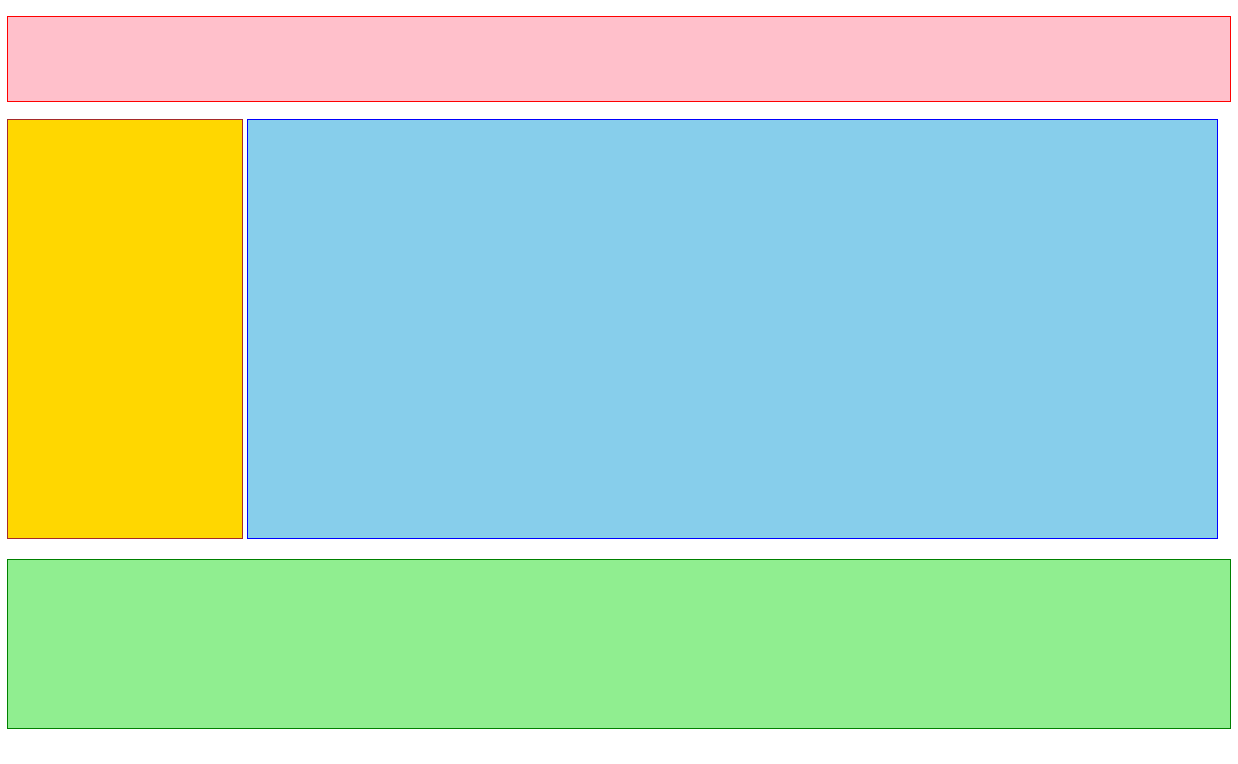
\includegraphics[width=\textwidth]{images/css-designing-html/exercise-responsive-2-wide.png}
        \caption{Wider than 800px}
        \label{fig:exercise-responsive-2-wide}
    \end{subfigure}
    \begin{subfigure}{.21\textwidth}\centering
        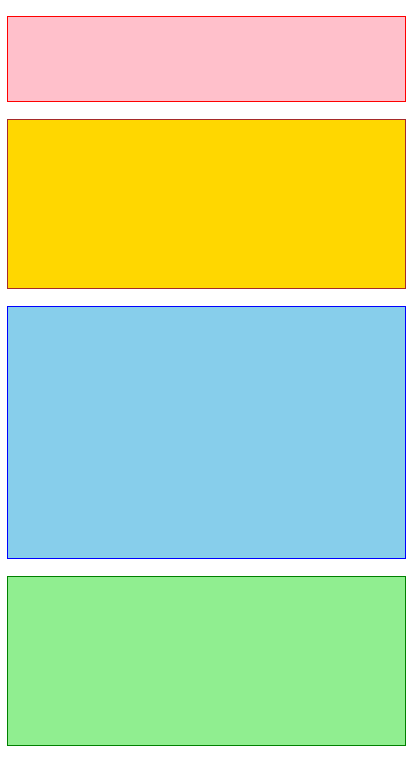
\includegraphics[width=\textwidth]{images/css-designing-html/exercise-responsive-2-small.png}
        \caption{Smaller than 800px}
        \label{fig:exercise-responsive-2-small}
    \end{subfigure}
    \caption{Webpage view of Exercise}
    \label{fig:exercise-responsive-2}
\end{figure}

\begin{codeenv}{code:exercise-responsive-web-2}{Exercise 5}\begin{verbatim}


<!doctype html>
<html>
<head>
    <title>CSS Exercise 5</title>
    <meta charset="utf-8">
    <meta name="viewport" content="width=device-width, initial-scale=1" >
    <link rel="stylesheet" text="type/css" href="./style.3.5.css">
</head>
<body>
    <div class="header"></div>
    <div class="body">
        <div class="navbar"></div>
        <div class="content"></div>
    </div>
    <div class="footer"></div>
</body>
</html>
\end{verbatim}
\end{codeenv}
